\documentclass[12pt]{article}
\usepackage[margin=1in]{geometry}
\usepackage{amsmath,amssymb,amsthm,booktabs,graphicx,natbib,microtype,array}
\newtheorem{theorem}{Theorem}
\newtheorem{corollary}[theorem]{Corollary}
\newtheorem{proposition}[theorem]{Proposition}
\newtheorem{remark}[theorem]{Remark}
\title{Sharp Stability Radii for Thresholded Packet Branches\\\large Clipped Singular-Value Selection and Projected-Cross Perturbations}
\author{Prime Dynamics Theory Program}
\date{July 2026}

\begin{document}
\maketitle

\begin{abstract}
Adaptive packet updates choose a width by comparing projected-cross singular
values with a relative threshold.  This branch is discontinuous at contact,
so an interval packet chain requires an explicit stability radius.  Let
$s_1\geq\cdots\geq s_M\geq0$, choose
\[
 w=\max\{m,\min(M,\#\{j:s_j/s_1\geq\tau\})\},
\]
and perturb the cross operator by at most $\varepsilon$.  We prove that the
clipped width is unchanged whenever
\[
 \varepsilon<\varepsilon_*=
 \min\left\{
 \frac{s_w-\tau s_1}{1+\tau}\ (w>m),\quad
 \frac{\tau s_1-s_{w+1}}{1+\tau}\ (w<M)
 \right\}.
\]
The omitted terms at the clipping endpoints are genuinely irrelevant.  Each
constant is sharp by a diagonal singular-value perturbation, and the radius
vanishes exactly at threshold contact.

For packet projectors we additionally prove
\[
 \|(I-P)AP-(I-Q)BQ\|
 \leq\|A-B\|+2\|B\|\|P-Q\|.
\]
This provides the interface from snapshot/projector balls to the singular
branch radius.  Auditing all three RH-96 thresholds gives 360/360 strict
branches and exact agreement with the archived widths.  Every branch also
dominates a conservative local fp64 proxy $128u n\|K\|$; the smallest ratio
is above $2388$.  Nevertheless the primary minimum relative branch radius is
only $4.3449\times10^{-9}$.  Thus local numerical branching is robust, but a
full source-to-update interval enclosure is not yet proved.
\end{abstract}

\section{Why width selection needs its own theorem}
RH-142 fixes the rank-four source projector at all ten frozen anchors.  The
recursive packet algorithm has another discontinuity: it selects two, three,
or four enrichment directions from the singular values of a projected
cross.  A small perturbation can change this integer branch even when the
underlying packet subspace varies continuously.  Once the branch changes,
the dimensions of the Ritz basis and all subsequent formulas change.

The correct certificate is not a derivative of the selected singular
vectors.  It is an open ball on which the inequalities defining the width
retain their signs.  Weyl's singular-value inequality makes this radius
explicit and dimension free \citep{StewartSun1990}.

\section{Sharp clipped branch radius}
Let $C$ be a nonzero operator with singular values
$s_1\geq\cdots\geq s_M$.  Fix a relative threshold $\tau\geq0$, a minimum
width $m$, and maximum width $M$.  The policy counts ratios above threshold
and clips the result into $[m,M]$.

\begin{theorem}[Threshold branch ball]\label{thm:branch}
Let $\widetilde C$ satisfy $\|\widetilde C-C\|\leq\varepsilon$.  If
$\varepsilon<\varepsilon_*$, where
\[
 \varepsilon_*=min\left(
 \left\{\frac{s_w-\tau s_1}{1+\tau}:w>m\right\}
 \cup
 \left\{\frac{\tau s_1-s_{w+1}}{1+\tau}:w<M\right\}
 \right),
\]
then the clipped threshold policy selects the same width $w$ for
$\widetilde C$.  Empty sides of the minimum are omitted.
\end{theorem}

\begin{proof}
Weyl's inequality gives
$|\widetilde s_j-s_j|\leq\varepsilon$.  For a non-minimum selected width,
the last retained ratio remains above threshold if
\[
 s_w-\varepsilon>\tau(s_1+\varepsilon),
\]
which is exactly the first radius condition.  For a non-maximum width, the
first omitted ratio remains below threshold if
\[
 s_{w+1}+\varepsilon<\tau(s_1-\varepsilon),
\]
which is the second.  Together they preserve the count after clipping.
When $w=m$, downward crossing of the $m$th value cannot reduce the clipped
width; when $w=M$, upward motion beyond the recorded block cannot increase
it.  Those inequalities are therefore unnecessary.
\end{proof}

\begin{proposition}[Sharpness]\label{prop:sharp}
Each finite term in $\varepsilon_*$ is best possible using only the displayed
singular values and an operator-norm perturbation.
\end{proposition}
\begin{proof}
For a retained wall, take a diagonal matrix and decrease $s_w$ by
$\varepsilon$ while increasing $s_1$ by $\varepsilon$.  At the stated radius
their ratio equals $\tau$.  For an omitted wall, increase $s_{w+1}$ and
decrease $s_1$ by the same amount.  Again equality occurs at the formula.
An arbitrarily larger perturbation crosses the branch.  These diagonal
changes have operator norm $\varepsilon$.
\end{proof}

At exact contact $s_j=\tau s_1$, the open radius is zero.  No continuous
single-valued branch certificate exists there; a set-valued policy or a
tie-breaking convention would be required.

\section{From projectors to the cross operator}
For a Hermitian memory Gram $A$ and packet projector $P$, define the ambient
projected cross
\[
 K(A,P)=(I-P)AP.
\]
Its nonzero singular values are the same as those obtained from any
orthonormal packet frame, so the threshold policy is basis invariant.

\begin{theorem}[Projected-cross perturbation]\label{thm:cross}
For Hermitian $A,B$ and orthogonal projectors $P,Q$,
\[
 \|K(A,P)-K(B,Q)\|
 \leq\|A-B\|+2\|B\|\|P-Q\|.
\]
\end{theorem}
\begin{proof}
Insert $K(B,P)$ and use
\[
 K(A,P)-K(B,P)=(I-P)(A-B)P,
\]
while
\[
 K(B,P)-K(B,Q)=(Q-P)BP+(I-Q)B(P-Q).
\]
Taking norms proves the formula.
\end{proof}

The coefficient two is the price of moving both the input and output packet
legs.  This bound is intentionally projector level; it avoids arbitrary
basis rotations inside the selected packet.

\section{RH-96 branch audit}
The RH-96 archive contains 120 updates at each threshold
$10^{-8},10^{-6},10^{-4}$.  For every step we recompute $w$ and
$\varepsilon_*/s_1$ from the first four projected-cross singular values.
All 360 widths agree exactly with the archive, and all 360 radii are positive.

\begin{table}[t]
\centering
\scriptsize
\begin{tabular}{ccccc}
\toprule
$\tau$ & strict branches & minimum relative radius & median radius & minimum / fp64 proxy\\
\midrule
$10^{-8}$ & $120/120$ & $4.345\times10^{-9}$ & $1.347\times10^{-2}$ & $2388.6$\\
$10^{-6}$ & $120/120$ & $3.227\times10^{-8}$ & $1.347\times10^{-2}$ & $17739$\\
$10^{-4}$ & $120/120$ & $3.236\times10^{-6}$ & $1.337\times10^{-2}$ & $8.89\times10^5$\\
\bottomrule
\end{tabular}
\caption{Finite threshold-branch margins.  The fp64 column is a local
backward-error proxy, not a source-model interval enclosure.}
\label{tab:audit}
\end{table}

The tight primary step is the left channel at $\sigma=0.08$, time six.  Its
normalized singular values are approximately
\[
 (1,0.2602,5.456\times10^{-4},5.655\times10^{-9}),
\]
so width three is protected mainly by the omitted fourth value's distance
below $10^{-8}$.  The margin is positive but far smaller than a typical
branch radius in the archive.

For numerical context only, we compare each relative radius with
$128u n$, where $u$ is binary64 unit roundoff and $n$ the ambient dimension.
Every decision passes by at least three orders of magnitude.  This confirms
that the archived width pattern is not a floating tie.  It does not certify
the errors inherited from an interval source state and moving packet.

\begin{figure}[t]
\centering
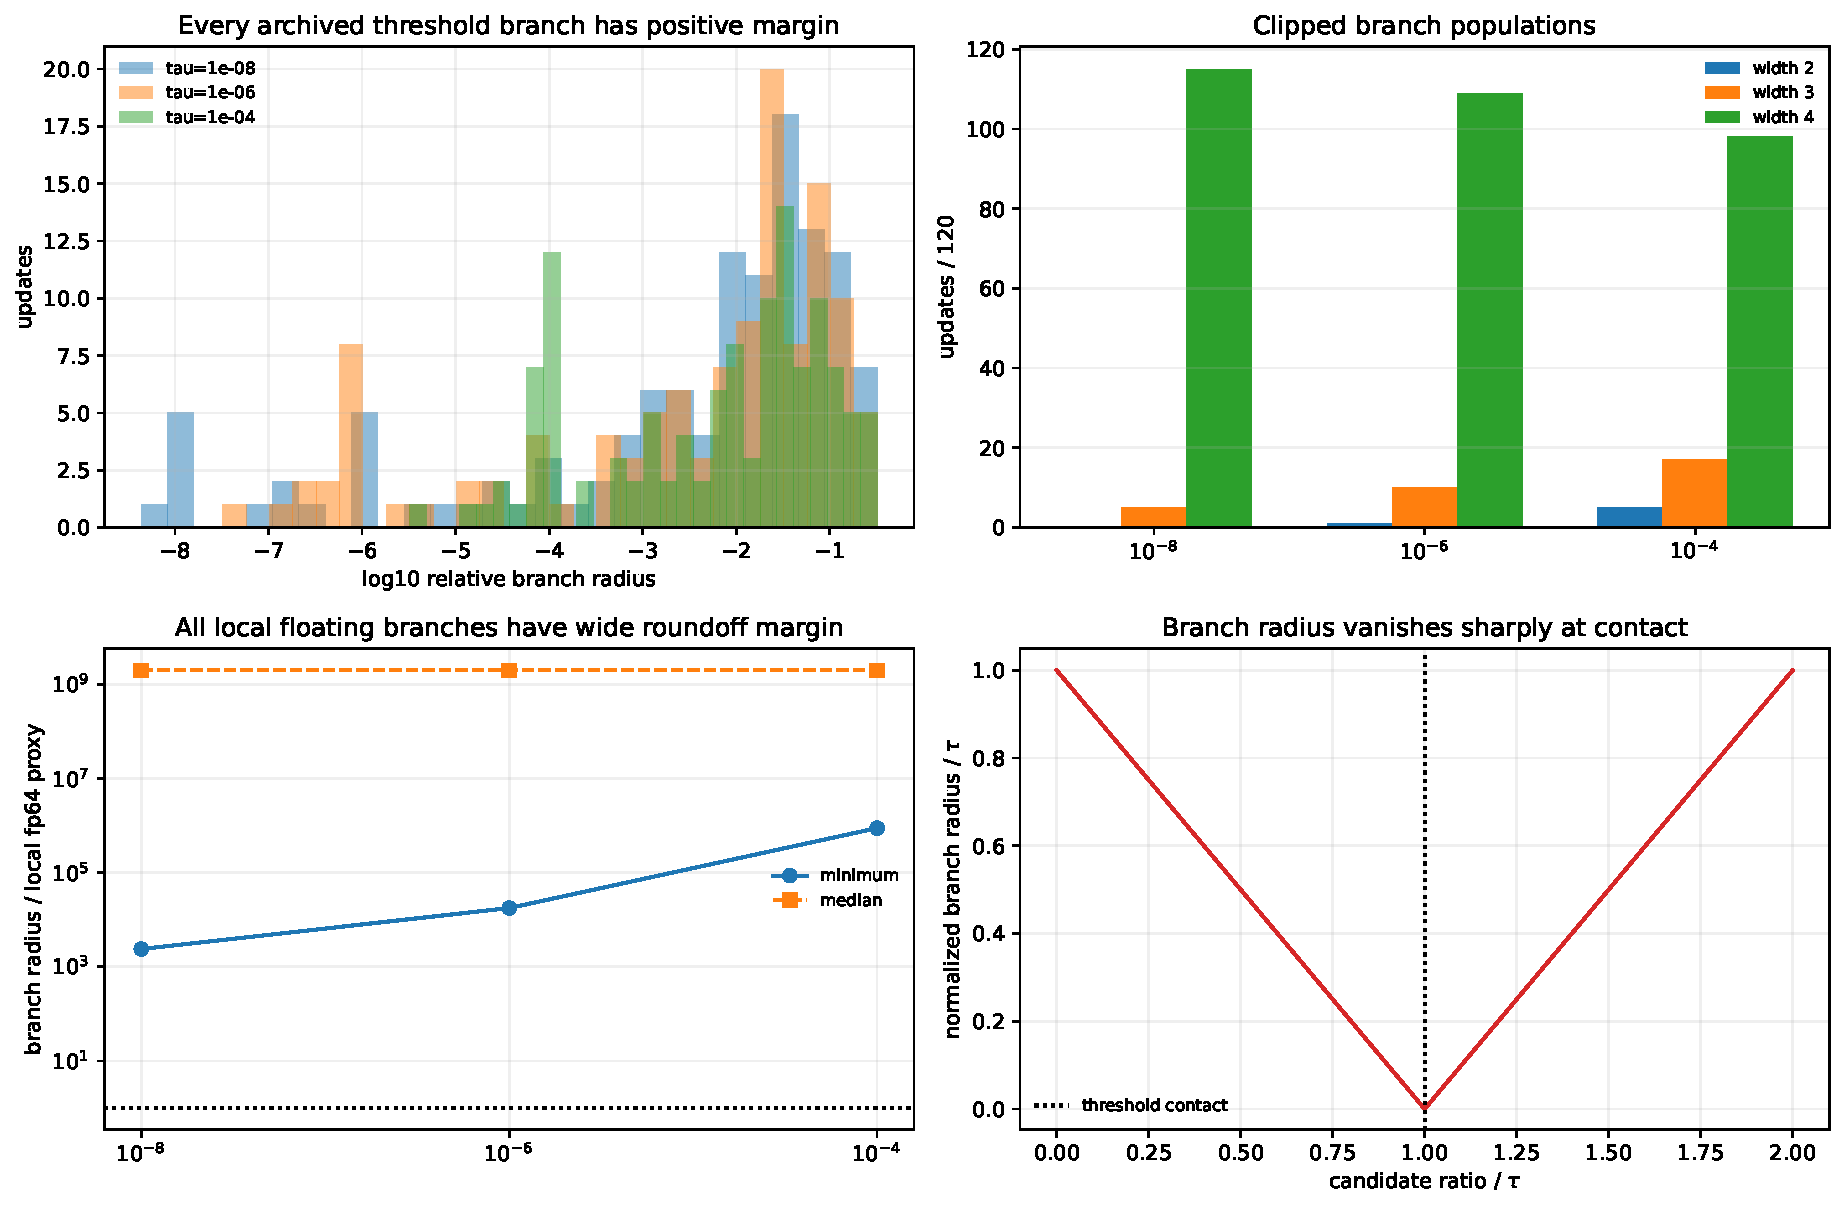
\includegraphics[width=\textwidth]{figures/threshold_branch_stability.pdf}
\caption{Branch-radius distributions, width populations, local roundoff
margins, and the sharp loss of stability at threshold contact.}
\label{fig:audit}
\end{figure}

\section{Consequence and claim boundary}
The exact condition for a validated update is now modular.  If a snapshot
and packet enclosure gives
\[
 \delta_A+2\|\widehat A\|\delta_P<\varepsilon_*,
\]
then Theorems~\ref{thm:cross} and \ref{thm:branch} freeze the adaptive width;
one may then enclose the fixed-dimensional Ritz/polar branch.  If this
inequality fails, the archived width cannot simply be assumed.

The broad coarse packet ball of RH-142 cannot yet be inserted blindly into
this inequality, and no temporal source-to-cross interval radii have been
computed.  We have not propagated all recursive packet updates, proved a
uniform threshold margin, closed controlled viability or the normalized-base
liminf, established Stage A, constructed a Hilbert--Polya operator, identified
zeta zeros, or proved the Riemann Hypothesis.

\bibliographystyle{plainnat}
\bibliography{references}
\end{document}
